%%
%% $Id$
%%
%% Copyright (c) 2007-2008 Christian Fehler
%% Copyright (c) 2007-2008 Benjamin Mies
%%


\chapter{Interaktion}\label{Interaction}

In diesem Kapitel wird die Interaktion mit dem Benutzer erläutert. Ein wichtiger
Aspekt der Interaktion ist, dass angezeigt wird, wenn etwas Falsches eingegeben
wurde. Ein weiterer Punkt ist, dass bei einem nicht deterministischen
Kellerautomaten auswählt werden muss, welchen Übergang der Automat machen soll,
da dieser das nicht in jedem Fall erkennen kann.\vspace{10pt}


\section{Fehler und Warnungen}\label{InteractionErrorWarning}

Es war uns bei der Umsetzung des \gtitools sehr wichtig, dass man als sehr viele
Fehler machen kann, ohne dass er durch eine Validierung eingeschränkt wird. Eine
Ausnahme von diesem Konzept bilden die in Kapitel \ref{Parser} beschriebenen
Parser, da eine falsche Eingabe dort nicht gut, durch das Anzeigen von Fehlern
bzw. Warnungen, behandelt hätte werden können.\vspace{10pt}

Der Hauptgrund für die Auswahl dieser Strategie war, dass der Benutzer durch das
fehlerhafte Eingeben bzw. durch das Beheben der Fehler hoffentlich mehr lernt,
als wenn er die Eingaben gar nicht erst hätte machen können. In diesem Abschnitt
werden die verschiedenen Fehler und Warnungen beschrieben, die bei Grammatiken und
Automaten auftreten können.\vspace{10pt}


\subsection{Grammatik}\label{InteractionGrammar}

Im Folgenden möchten wir auf die Fehler und Warnungen eingehen, welche bei dem
Validierungsvorgang einer Grammatik auftreten können.\vspace{10pt}

Zu diesen Validierungsfehlern zählt unter anderem wenn Produktionen mehrfach
in einer Grammatik existieren. In der Spalte "`Meldung"' sieht man wie immer
nur, um welchen Fehler es sich gerade handelt. Über die Beschreibung wird
mitgeteilt, um welche Produktion es sich dabei handelt. Man kann sich die
betreffenden Produktionen auch farblich hervorheben lassen, indem man die
entsprechende Fehlermeldung durch Mausklick auswählt. So kann der Benutzer die
fehlerhaften Produktionen schnell lokalisieren und den Fehler beheben.\vspace{10pt}

Handelt es sich bei der aktuellen Grammatik um eine reguläre Grammatik, gibt es
noch eine weitere Fehlermeldung. Wenn nicht alle Produktionen den vorgegebenen
Satzformen für eine rechtsreguläre Grammtik entsprechen, wird dies auch durch
einen Validierungsfehler angezeigt. Dabei kann man auch hier anhand der
Beschreibung sehen, um welche Produktion es sich handelt. Wenn man den
entsprechenden Eintrag auswählt, wird dem Benutzer wieder durch farbiges
Hervorheben signalisiert, wo sich diese Produktion befindet. Es wird jetzt
allerdings nicht die ganze Produktion eingefärbt, sondern nur der Teil der
Satzform, welcher nicht den Satzformen für reguläre Grammatiken entspricht. Auch
hier war wieder die Intention, dem Benutzer schnell zu einer gültigen Grammatik
zu verhelfen.\vspace{10pt}

Neben diesen beiden Fehlern haben wir auch eine Warnung eingeführt. Diese gibt
Auskunft darüber, wenn ein Nichtterminalzeichen, vom Startsymbol ausgehend, nicht
Teil einer ableitbaren Satzform ist. Es handelt sich hierbei nur um eine Warnung,
weil es sich durchaus um eine gültige Grammatik handeln kann. Sie soll dem
Benutzer allerdings dazu animieren, die Produktionsmenge zu kontrollieren, ob
nicht eine oder mehrere Produktionen vergessen wurden. So soll es möglich sein,
Flüchtig\-keits\-fehler frühzeitig zu erkennen und zu beheben.\vspace{10pt}

\subsection{Automat}\label{InteractionMachine}

Auch für Automaten gibt es einige Fehler und Warnungen die nun aufgezählt
werden. Die verschiedenen Automatentypen verwenden unterschiedliche Fehler. So
ist ein $\epsilon$-Übergang in einem $\epsilon$-NDEA kein Fehler, in einem DEA
aber schon. Deshalb wird bei jedem Fehler angegeben, in welchem Automaten er
auftreten kann.\vspace{10pt}

\noindent
\begin{tabular}{|p{2.1cm}|p{2.7cm}|p{6.0cm}|}
  \hline
  \textbf{Meldung} &
  \textbf{Automaten} &
  \textbf{Beschreibung} \\
  \hline
  \hline
  Alle Symbole &
  DEA &
  Ein Zustand muss Übergänge mit allen Symbolen enthalten \\
  \hline
  Symbole nur einmal &
  DEA und Kellerautomat &
  Ein Zustand darf nicht mehrere Übergänge mit dem gleichen Symbol enthalten \\
  \hline
  $\epsilon$-Übergang &
  DEA und NDEA &
  Es darf kein $\epsilon$-Übergang vorhanden sein \\
  \hline
  Keller-Operationen &
  DEA, NDEA und $\epsilon$-NDEA &
  Es dürfen keine Operationen auf dem Keller ausgeführt werden \\
  \hline
  Mehr als ein Start-Zustand &
  DEA, NDEA, $\epsilon$-NDEA und Kellerautomat&
  Es darf nur ein Start-Zustand vorhanden sein \\
  \hline
  Kein Start-Zustand &
  DEA, NDEA, $\epsilon$-NDEA und Kellerautomat&
  Es muss ein Start-Zustand vorhanden sein \\
  \hline
  Eindeutiger Zustandsname &
  DEA, NDEA, $\epsilon$-NDEA und Kellerautomat&
  Die Namen der Zustände müssen eindeutig sein \\
  \hline
\end{tabular}
\vspace{10pt}

\noindent
Neben diesen Fehlern gibt es auch noch zwei Warnungen. Zum einen wird der
Benutzer gewarnt, wenn kein akzeptierender Zustand vorhanden ist. Dabei handelt
es sich nicht um einen ungültigen Automaten, aber es könnte sein, dass der
ungeübte Benutzer den akzeptierenden Zustand nur vergessen hat. Außerdem wird
eine Warnung angezeigt, wenn ein oder mehrere Zustände nicht erreichbar sind.
Zur Bestimmung dieser unerreichbaren Zustände wird der in Kapitel
\ref{ReachableStates} beschriebene Algorithmus benutzt.\vspace{10pt}


\section{Operationen mit dem Automaten Keller}\label{InteractionPDA}

Ein wichtiger Punkt der Interaktion mit dem Benutzer ist, dass der Benutzer nach
einer Umwandlung einer kontextfreien Grammatik in einen nicht deterministisch
Kellerautomaten einen Übergang auswählen muss, weil der entstehende Automat
nicht deterministisch sein muss. Die Umwandlung ist in Abschnitt
\ref{ConverToGrammarContextFree} zu finden.\vspace{10pt}

\begin{figure}[h!]
\begin{center}
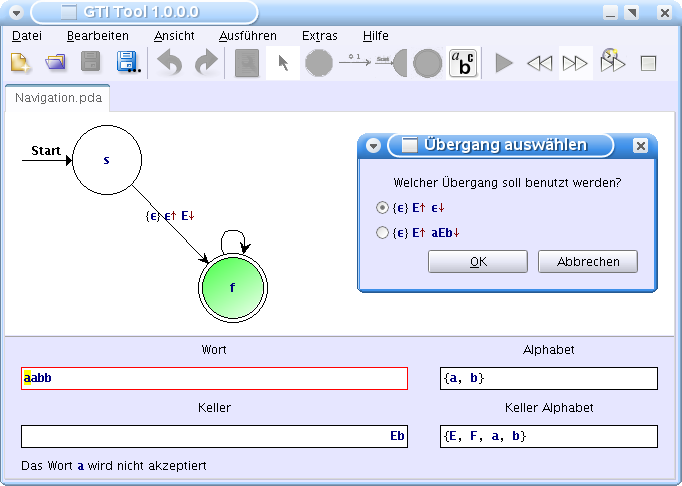
\includegraphics[width=12cm]{../images/grammar_pda.png}
\caption{Operationen mit dem Automaten Keller}
\label{FigureGrammarPDA}
\end{center}
\end{figure}
\vspace{10pt}

Bei dem in Abbildung \ref{FigureGrammarPDA} verwendeten Beispiel kommen zwei
Übergänge in Frage: Es könnte der Übergang gewählt werden, der \Symbol{E} vom
Keller liest und nichts auf diesen schreibt, oder aber der Übergang, der
\Symbol{E} vom Keller liest und \Symbol{a}\Symbol{E}\Symbol{b} auf ihn schreibt.
Da \Symbol{a} als nächstes auf dem Eingabeband steht, sollte der zweite Übergang
ausgewählt werden, da bei der Verwendung des ersten Übergangs das \Symbol{a}
nicht mehr herleitbar ist. Dem Benutzer steht es allerdings frei, auch den
anderen Übergang auszuwählen. In diesem Fall würde das Wort
\Symbol{a}\Symbol{a}\Symbol{b}\Symbol{b} aber nicht akzeptiert werden. Der
Benutzer hat bei einer Wahl, die sich im Nachhinein als falsch herausstellt,
allerdings die Möglichkeit, einen oder mehrere Schritte zurückzugehen, um dann
die hoffentlich richtige Wahl zu treffen.\vspace{10pt}
